\documentclass[a4paper]{article}
\usepackage{pdflscape}
\setlength\marginparwidth{0in}
\setlength\marginparsep{0in}
\usepackage[left=1in, right=1in, top=1in, bottom=1in]{geometry}
\usepackage{lipsum}
\usepackage{graphicx}
%% \graphicspath{./images}
\usepackage{fancyhdr}
\pagestyle{fancy}
\fancyfoot{}
\renewcommand{\headrulewidth}{0pt}
\fancyfoot[RO]{\footnotesize \sc From the Mahatma Gandhi Centennial Collection of Ramakant D.\ Bhat-Upponi (1927--1996)}
\begin{document}
\begin{landscape}
  \hrule
  \vspace{8pt}
  \begin{minipage}{5cm}
    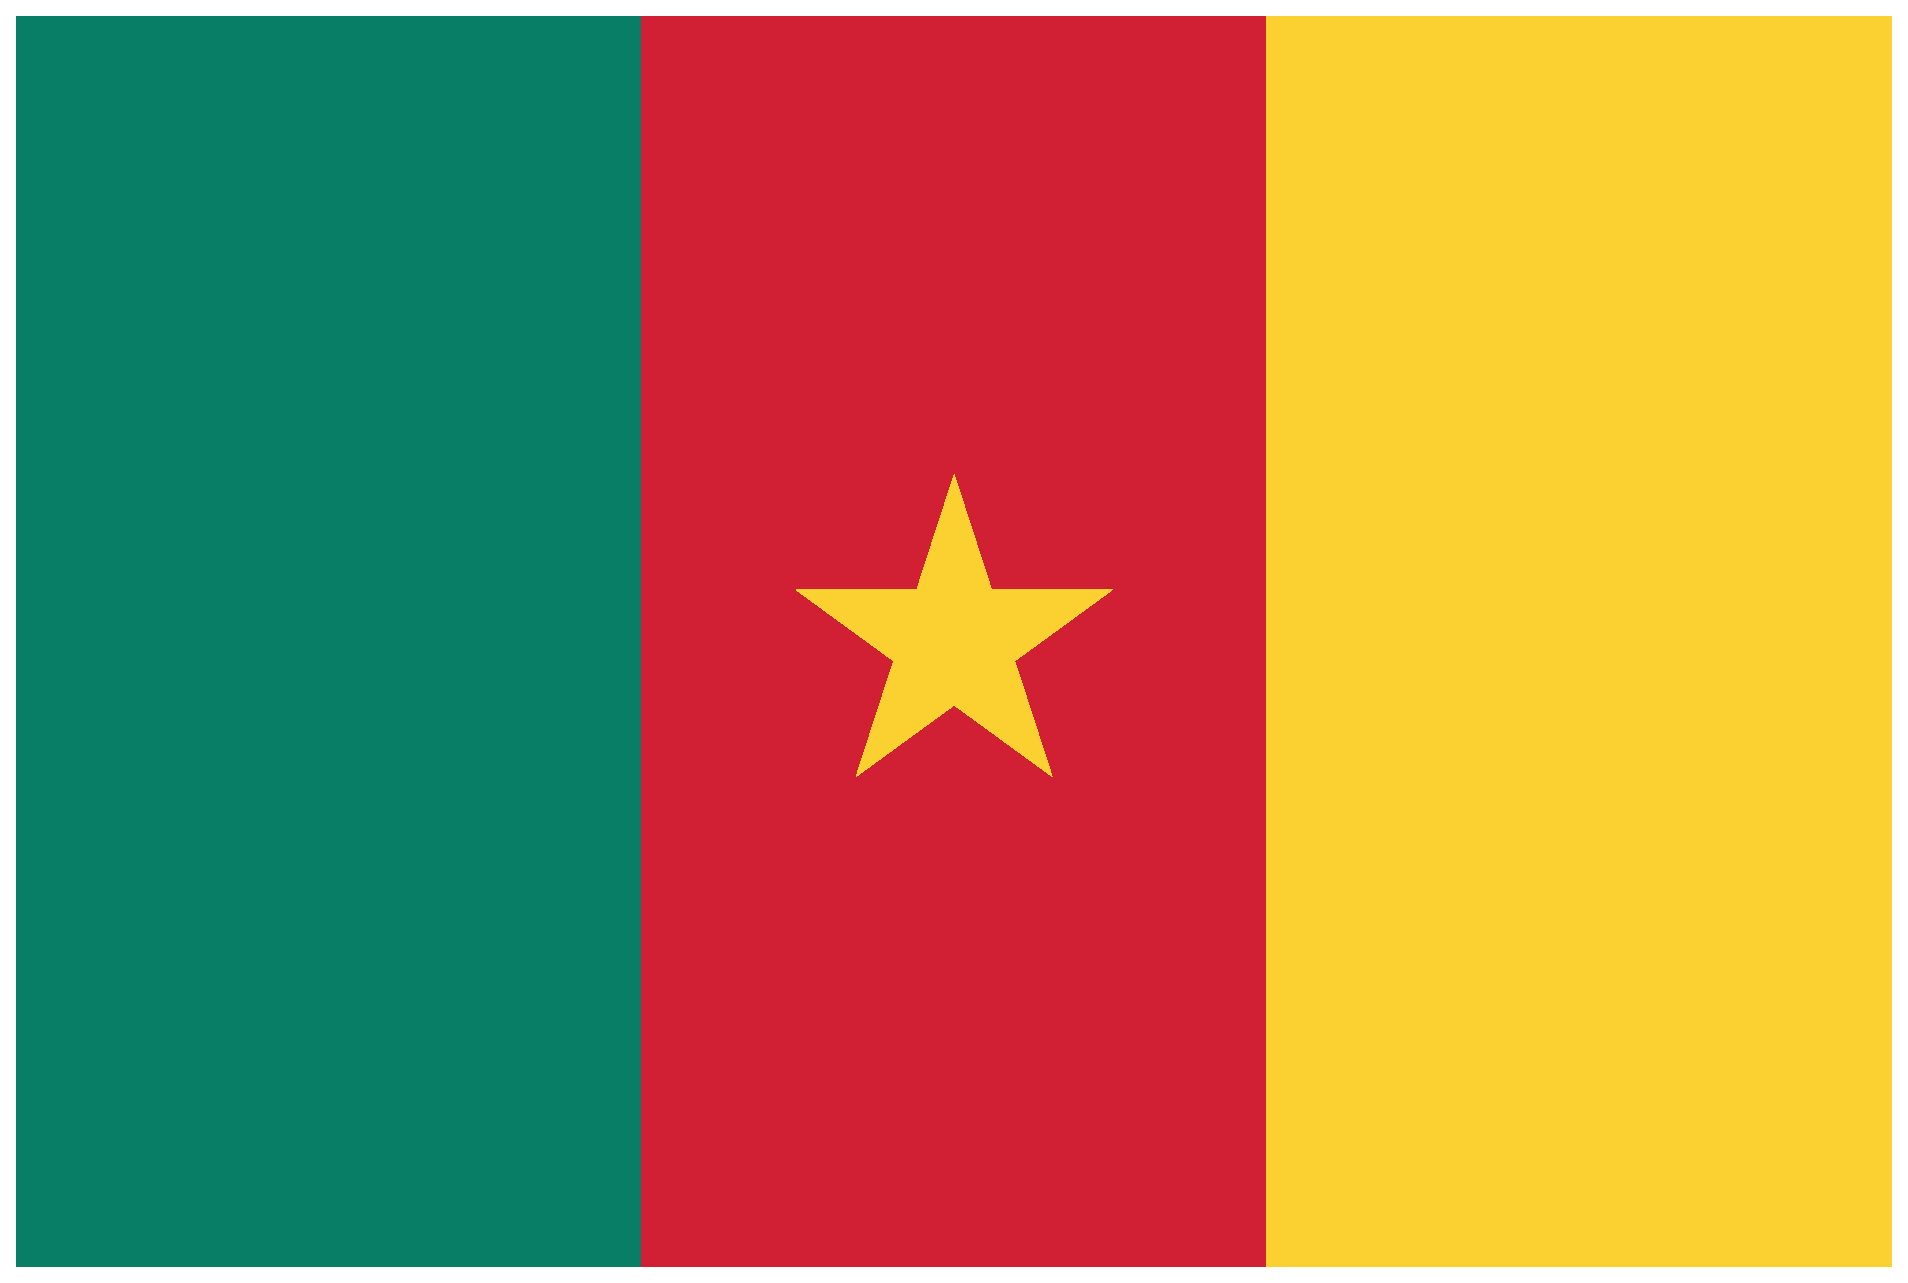
\includegraphics[height=1.2cm]{images/cm}
  \end{minipage}
  \hfill
  {\scshape\Huge Federal Republic of Cameroon}
  \vspace{8pt}
  \hrule
  \vspace{11.5cm}
  \begin{center}
    \begin{minipage}{17cm}
      \hrule \vspace{12pt} Cameroon issued a set of two stamps honouring
      the Mahatma on December 5, 1968. Issued as a {\it se-tenant} (a
      block of different stamps or labels), each pair is separated by a
      stamp-size label with his name, years of birth and death and the
      words ``Advocates of Non-Violence''. In addition, Cameroon also
      issued a First Day Cover, Imperfs (un-perforated stamps), deluxe
      cards, souvenir sheets (both thick and thin) in this batch.
    \end{minipage}
  \end{center}
\end{landscape}
\end{document}
